\chapter{Referencial Teórico}\label{cap:refTeor}

Será abordado neste capítulo o conteúdo base na compreensão deste trabalho dividido em 3 sessões: Aprendizado de Máquina, Discretização e Trabalhos Correlatos. 

A primeira sessão contempla os principais tipos de aprendizados indutivos, não incluindo aqui o aprendizado semi-supervisionado e sim dando ênfase a aprendizagem supervisionado, foco da proposta deste mestrado. O aprendizado indutivo utiliza uma amostra do todo para tirar uma conclusão. Caso os exemplos retirados de uma base de dados não forem suficientes, talvez o conhecimento derivado destes exemplos não mostrem a verdade. 

O segundo ítem dissertará sobre a técnica de discretização adotada nesta pesquisa. Possuindo grande contribuição para os resultados gerados, e ganhando assim uma sessão própria para explanação de como funciona essa técnica. E na terceira sessão serão abordados trabalhos com mesmas características particulares para melhor elucidar o motivo da elaboração dessa proposta de mestrado.



\section{Aprendizado de Máquina}\label{sec:aprendMaq}

Aprendizagem de máquina é a capacidade do aprendizado automático com utilização de algoritmos atuando em cima de uma base de dados.  Diz-se que o computador está aprendendo quando existe uma melhora de desempenho de tarefas que ele utilizou como exemplo \cite{Mitchell1997}. Um exemplo seria a realização do reconhecimento facial de uma pessoa utilizando aprendizado de máquina. Não seria necessário a implementação de várias linhas de código informando que a cor do olho é azul, a orelha e cabelo grandes seriam de uma certa pessoa. Ao invés disso é observada várias fotos tituladas de uma certa pessoa, e após vários exemplos o computador seria capaz de predizer uma foto nova, se é, ou não, da determinada pessoa através de aprendizado anterior.

Existem alguns motivos, onde justificam, que não é possível simplismente exigir que o projetista implemente melhorias no sistema de forma que ele esteja robusto bastante para lidar com todas as situações \cite{RusselStuart.Norvig2013}. Um  desses motivos seria a incapacidade da antecipação de  todas as situações possíveis de implementação por parte do programador. Fazendo um resumo, aprendizado de máquina seriam algoritmos capazes de aprender automaticamente através de  determinados exemplos, ou comportamentos. 

A partir desta síntese, tem-se uma observação. A classificação de dados no contexto de aprendizado de máquina, compostos por dois pilares. Um, seriam os dados a serem classificados, e outro o algoritmo que irá atuar nessa base de dados. Existem vários algoritmos como exemplo: redes neurais, árvores de decisão, Suport Vector Machine – SVM, etc. Qualquer um destes algoritmos são utilizados para solucionar essa classificação. E a escolha apropriada, desse algoritmo, se dará através de métricas que avaliaram o desempenho de cada um, e a melhor métrica, será o algoritmo apropriado para aquele problema de classificação de dados. 

Uma analogia referente do que foi dito acima seria um “problema” qualquer sendo comparado a um “motor”, e os algoritmos disponíveis seriam as ferramentas para concertar esse motor. A partir daí a ferramenta que fosse mais eficaz, considerando métricas de desempenho, para fazer o motor funcionar, seria a ferramenta(algoritmo) escolhida. Tendo assim a escolha certa para um determinado problema.

\subsection{Aprendizado Supervisionado}\label{ssec:aprendSup}

Nesta sessão será abordado um método que através de uma banco de dados já classificado por especialistas, será feita uma predição de novos registros com base em vários desses exemplos já classificados. Os responsáveis por essas predições de novos registros são algoritmos de aprendizado supervisionados projetados para determinados fins.


O termo "Supervisionado" indica que existe um supervisor para cada registro de entrada especificando uma saída para esse registro. Considerando uma base de dados de imagens de rostos, onde cada imagen possui uma saída representado por uma classe: masculino ou feminino. A tarefa seria criar um preditor capaz de acertar a cada novo registro se a imagem é masculina ou feminina. Seria  difícil  implementar de maneira tradicional, uma vez que são inúmeras as diferenças que difere as faces masculinas e femininas. Mas uma alternativa seria dar exemplos de rostos com suas classificações de fazer que automaticamente a máquina "aprenda" uma regra para predizer se é masculino ou feminino \cite{Barber2011}.

Em \cite{RusselStuart.Norvig2013} os autores fazem uma apresentação formal do funcionamento da aprendizagem supervisionada. Dado um conjunto de treinamento 
\begin{equation}
 (x_{1},y_{2}),(x_{2},y_{2}),...(x_{n},y_{n}),
 \label{eq:aprendSup}
\end{equation}
onde cada ${y_{j}} $ foi gerado por ${y=f(x)}$ desconhecida. Encontrar uma função ${h}$ que se aproxime da função ${f}$ real.

A função ${h}$ é uma hipótese onde prevê um melhor desempenho entre as hipóteses possíveis através dos conjuntos de exemplos, que são diferentes do conjunto de treinamento \ref{eq:aprendSup}.

 \begin{figure}[h!]
    \centering
    \subfloat[Ajuste polinomial de grau 6]{
        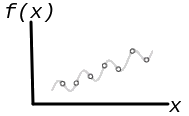
\includegraphics[scale=0.8]{figs/grafA.png}
        \label{fig:graf1:grafA} }
    \quad
    \subfloat[Hipótese linear]{
        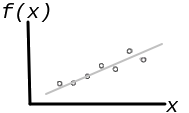
\includegraphics[scale=0.8]{figs/grafB.png}
        \label{fig:graf1:grafB} }
    
    \caption{Hipóteses ajustadas} \label{fig:graf1}
        
        %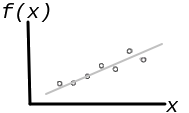
\includegraphics[scale=0.4]{figs/grafB.png}
        %\caption{Polinômio Superajustado} \label{grafB}
      \end{figure}

Na figura \ref{fig:graf1:grafA} existe um sobre ajuste da função com o conjunto de dados de treinamento. Acabou se tornando uma função mais complexa para se molda de acordo com os sete pontos do gráfico, especificando para esse conjunto de dados. 

Ja na figura \ref{fig:graf1:grafB} o ajuste da função se torna mais simples e mesmo não passando por todos os pontos. Mas acaba generalizando melhor o conjunto de treinamento tornando, talvez, um melhor resultado da predição de novos valores.

A figura \ref{fig:graf1} mostra duas hipóteses que tentam se aproximar ao máximo da função verdadeira. Então ${h}$ tem que generalizar bem, para prevê melhor os valores de ${y}$ para novos conjuntos de dados.

\subsubsection{Classificatio and Regression Trees - CART}\label{sssec:cart}


\subsubsection{Naive Bayes}\label{sssec:nbayes}


\subsection{Aprendizado Não Supervisionado}\label{ssec:aprendNSup}

No aprendizado não supervisionado, não existe uma tentativa de se encontrar uma função que se aproxime da real. Logo porque os registros não são classificados. Desta forma os algoritmos procuram algum grau de simularidade entre os registros e tenta agrupá-los de forma a ter algum sentido eles estarem juntos. 

Os números de clusters encontrados irão depender de como os algoritmos funcionam, junto com o grau de dissimilaridade entre elementos de grupos diferentes. Como não existe uma variável classe no aprendizado não supervisionado, então \cite{Barber2011} diz que o maior interesse seria em uma perspectiva probabilística de ditribuição ${p(x)}$ de um determinado conjunto de dados 
\begin{equation}
 D = \{x_{n},n=1,...,N\}
 \label{eq:aprendNSup}
\end{equation}
.


\section{Trabalhos Correlatos}\label{sec:primTrab}

Eu queria testar notas\footnote{Referente \cite{Mitchell1997}  } de rodapé\cite[Seilá]{Mitchell1997}. Ainda não sei como fazer.


\lipsum[34]
